\documentclass[10pt]{article}

%defines page size and margins
\usepackage{geometry}
\geometry{
    letterpaper,
    left=1in,
    right=1in,
    top=1in,
    bottom=1in,
}

%Sets spacing for entire document
\usepackage{setspace}
\singlespacing

%Package for reducing space in between list items
\usepackage{enumitem}

%Math symbols
\usepackage{gensymb}
\usepackage{siunitx}

%Image path
\usepackage{graphicx}
\graphicspath{ {/} }

%Used for adjusting images
\usepackage[export]{adjustbox}

%For floating images
\usepackage{float}

\begin{document}
\title{Laboratory Three --- AC Circuits}
\date{October 13, 2017}
\author{Rishabh Shah\\ 4655 4192\\ \\ Partner: Matthew Remillard}
\maketitle
\newpage

\section*{Pre-Lab}
\subsection*{I}
\noindent$$RiseTime = \frac{arcsin(0.8)}{pi \cdot Freq} = \frac{T \cdot arcsin(0.8)}{pi}$$

\noindent$$RiseTime(50 kHz) = \frac{arcsin(0.8)}{pi \cdot 50000} = 5.9033 \times 10^{-6}\mu s$$

\subsection*{II}
\noindent$$Measured Ratio of \frac{R_1}/{R_2} = \frac{R_1}{R_2} = \frac{V_1}{V_2} = \frac{1.5}{2} = 0.75$$

\noindent$$Calculated Ratio of \frac{R_1}/{R_2} = \frac{R_1}{R_2} = \frac{100}{200} = 0.5$$

\noindent$$Percentage Error = \frac{|measured-calculated|}{calculated} = \frac{|0.75-0.5|}{0.5} = 50\%$$

\subsection*{III}
\noindent$$V_{D0} = V_S - V_{out} = 4.850 - 608.74 \times 10^{-3} = 4.24V$$

\section*{Lab Data}
\begin{figure}[H]
	\centering
	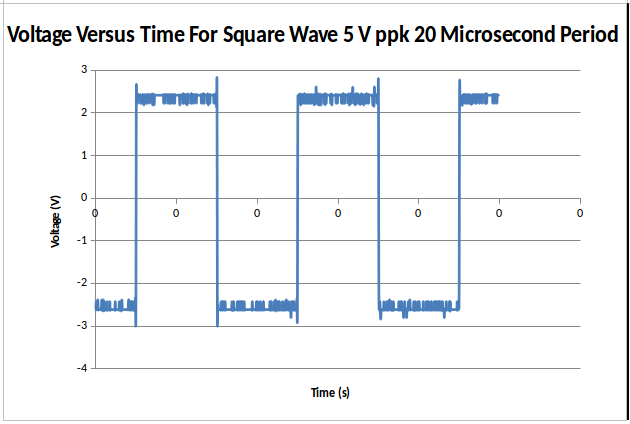
\includegraphics[width=\textwidth]{Square}
\end{figure}
\begin{figure}[H]
	\centering
	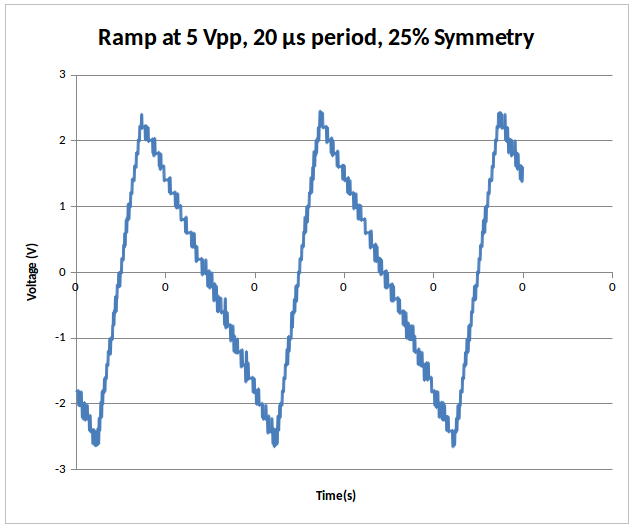
\includegraphics[width=\textwidth]{Ramp25}
\end{figure}
\begin{figure}[H]
	\centering
	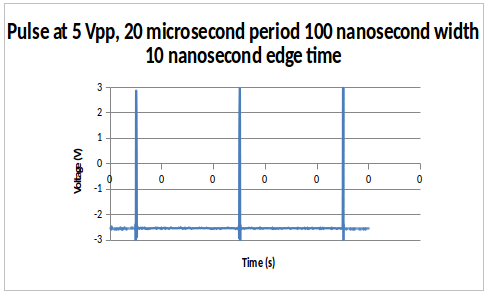
\includegraphics[width=\textwidth]{Pulse10}
\end{figure}
\begin{figure}[H]
	\centering
	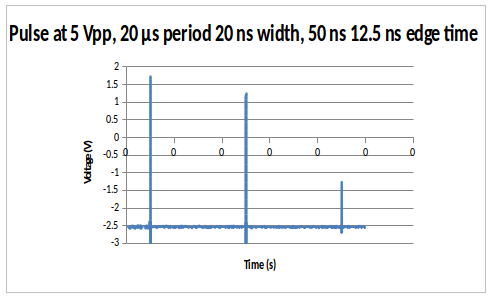
\includegraphics[width=\textwidth]{Pulse125}
\end{figure}
\begin{figure}[H]
	\centering
	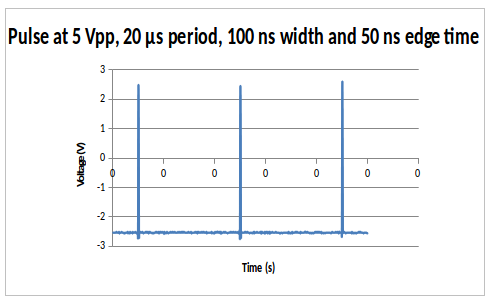
\includegraphics[width=\textwidth]{Pulse50}
\end{figure}
\begin{figure}[H]
	\centering
	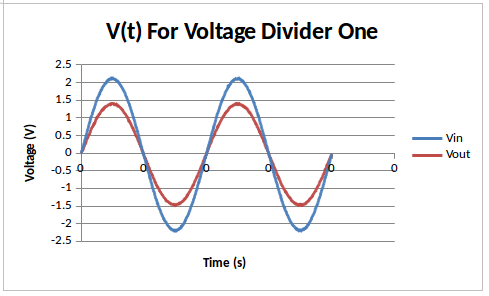
\includegraphics[width=\textwidth]{Divider1}
\end{figure}
\begin{figure}[H]
	\centering
	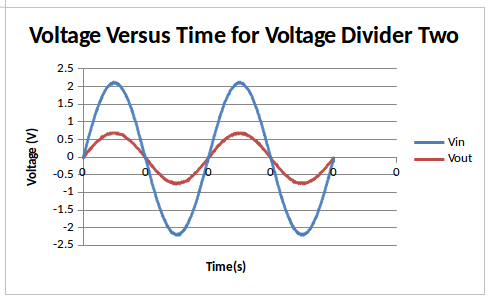
\includegraphics[width=\textwidth]{DividerTwo}
\end{figure}
\begin{figure}[H]
	\centering
	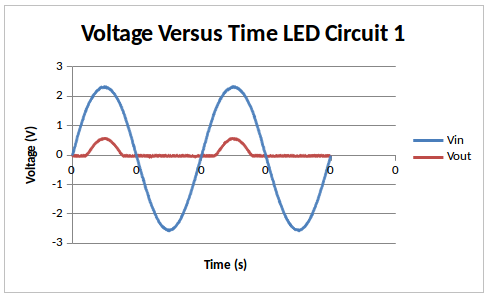
\includegraphics[width=\textwidth]{LED1}
\end{figure}
\begin{figure}[H]
	\centering
	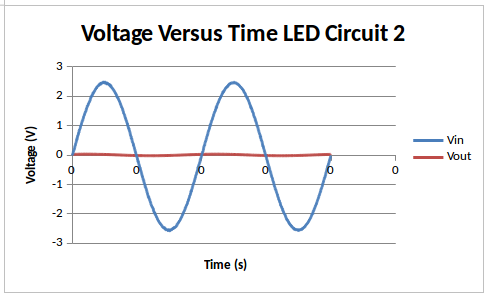
\includegraphics[width=\textwidth]{LED2}
\end{figure}
\begin{figure}[H]
	\centering
	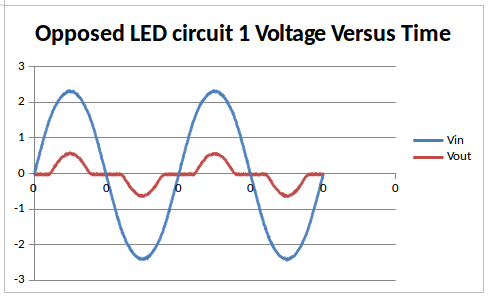
\includegraphics[width=\textwidth]{Opposed1}
\end{figure}
\begin{figure}[H]
	\centering
	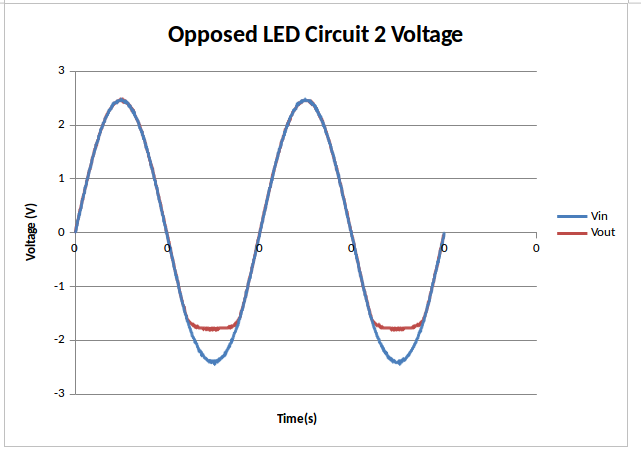
\includegraphics[width=\textwidth]{Opposed2}
\end{figure}
\begin{figure}[H]
	\centering
	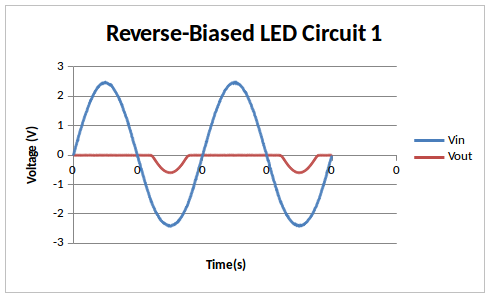
\includegraphics[width=\textwidth]{Reversed1}
\end{figure}

\section*{Post-Lab}
\subsection*{I}
\begin{table}[H]
	\centering
	\begin{tabular}{|l|l|l|}
		\hline
		 & \textbf{Fall Time (s)} & \textbf{Rise Time (s)} \\
		\hline
		\textbf{Calculated} & $5.9033 \times 10^{-6}$ & $5.9033 \times 10^{-6}$ \\
		\hline
		\textbf{Measured} & $5.8020 \times 10^{-6}$ & $5.8020 \times 10^{-6}$ \\
		\hline
	\end{tabular}
\end{table}

\noindent$$Percentage Error = \frac{|measured-calculated|}{calculated} = \frac{|5.8020 \times 10^{-6} - 5.9033 \times 10^{-6}|}{5.9033 \times 10^{-6}} = 1.7160\%$$

\subsection*{II}
\begin{table}[H]
	\centering
	\begin{tabular}{|l|l|l|l|l|l|}
		\hline
		 & \textbf{$V_S (V)$} & \textbf{$V_{out} (V)$} & \textbf{Voltage Ratio $V_S/V_{out}$} & \textbf{Theoretical Ratio} & \textbf{Percentage Error} \\
		\hline
		\textbf{Circuit 1} & $4.50$ & $2.93$ & $0.67$ & $0.6511$ & $2.33\%$ \\
		\hline
		\textbf{Circuit 2} & $4.50$ & $1.47$ & $0.33$ & $0.3267$ & $2.00\%$ \\
		\hline
	\end{tabular}
\end{table}

\subsection*{III}
\begin{table}[H]
	\centering
	\begin{tabular}{|l|l|l|}
		\hline
		\textbf{$V_S (V)$} & \textbf{$V_{out} (V)$} & \textbf{$V_{Offset} (V)$} \\
		\hline
		0 & 0.12 & n/a \\
		\hline
		1 & 0.12 & n/a \\
		\hline
		2 & 0.12 & n/a \\
		\hline
		3 & 0.12 & n/a \\
		\hline
		4 & 0.32 & 1.840 \\
		\hline
		5 & 0.68 & 2.160 \\
		\hline
		6 & 1.05 & 2.475 \\
		\hline
	\end{tabular}
\end{table}

The measured values seem quite far from our calculated offset voltage.

$$Percentage Error = \frac{|measured-calculated|}{calculated} = \frac{|2.475-4.24|}{4.24} = 41.6274\%$$

\noindent Since the diode will only allow current to flow through it if the current has a voltage larger than the forward voltage of the diode, and because it only allows current to flow one way, the current passing through will be DC.

\subsection*{IV}
\begin{table}[H]
	\centering
	\begin{tabular}{|l|l|l|}
		\hline
		 & \textbf{$V_S (V)$} & \textbf{$V_{out} (V)$} \\
		\hline
		\textbf{Circuit 1} & $5.100$ & $0.620$ \\
		\hline
		\textbf{Circuit 2} & $5.100$ & $4.400$ \\
		\hline
	\end{tabular}
\end{table}

\noindent Because the LED only allows current to flow through it if the current has a voltage larger than the forward voltage of the diode, and because it only allows current to flow one way, the LED does not allow current through in the first circuit, but does in the second circuit.

\subsection*{V}
\begin{table}[H]
	\centering
	\begin{tabular}{|l|l|l|}
		\hline
		 & \textbf{$V_S (V)$} & \textbf{$V_{out} (V)$} \\
		\hline
		\textbf{Circuit 1} & $4.82$ & $1.25$ \\
		\hline
		\textbf{Circuit 2} & $4.90$ & $1.78$ \\
		\hline
	\end{tabular}
\end{table}

\subsection*{VI}
\begin{table}[H]
	\centering
	\begin{tabular}{|l|l|l|l|l|l|}
		\hline
		 & \textbf{$V_S (V)$} & \textbf{$V_{out} (V)$} & \textbf{$Measured V_{offset} (V)$} & \textbf{$Theoretical V_{offset} (V)$} & \textbf{Percentage Error} \\
		\hline
		\textbf{Circuit 1} & $4.82$ & $1.25$ & $1.785$ & $1.7$ & $5.00\%$ \\
		\hline
		\textbf{Circuit 2} & $4.90$ & $1.78$ & $1.560$ & $1.7$ & $8.24\%$ \\
		\hline
	\end{tabular}
\end{table}

\noindent This does match our expectations because it is within 10\% of our theoretical values.

\end{document}